\chapter{RESULT}

\noindent\hspace{2.5em}We have used pre-recorded footage from CCTV cameras to analyze and compare the performance and accuracy of the detection and counting system. 

\vspace{1em}


\section{Model Result}
\noindent\textbf{Table 4.1} \\
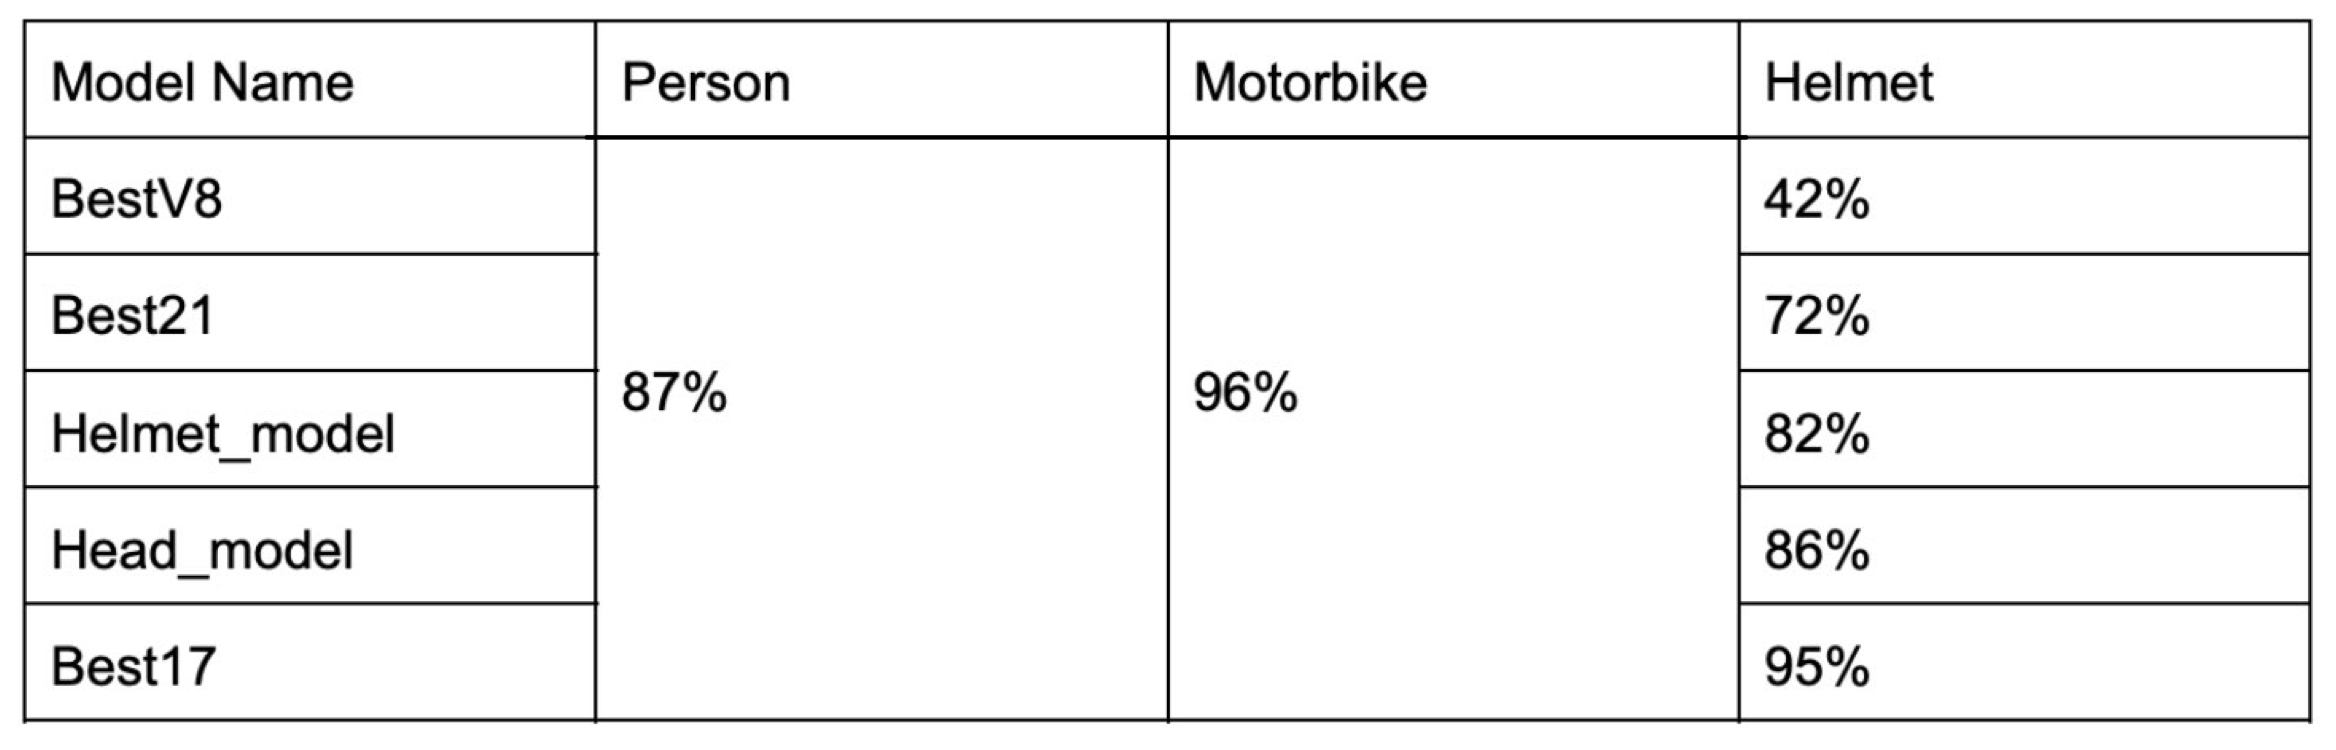
\includegraphics[width=1\textwidth]{table4.1.jpg}


\noindent\hspace{2.5em}To evaluate the accuracy of the model, we compared detection counts with manual counting over a ten-minute span of one video with every model we have. The aim of this is to see the accuracy and improvement of our model. The results in Table 4.1 shows the accuracy results of different models. Person and motorbike used YOLO pretrain model to detect these two classes, so the accuracy and considered constant throughout different models. Helmet detection rises from 42\% to 96\%, which is 54\% improvement from the first model to latest model. The calculation method of finding helemt detection accuracy across different models is to find the total ground truth and detection of the train model, then divide it to find the accuracy. We find the best confident for each model by comparing confident of 0.15 and 0.3 to find the best accuracy. Best17 model have the ground truth helmet of 60, we have the confident set to 0.15 and detected the detection number to be 55, which is 90\%. On the other hand, we change the confident to 0.3 and the results of the detection is 58, which is 95\% resulting in a better accuracy.

Table 4.1 presents the detection accuracy of various models across three object categories: person, motorbike, and helmet. The accuracy values for person and motorbike detection remain constant across models—87\% and 96\% respectively—because these classes were detected using the pretrained YOLO model without additional fine-tuning. In contrast, the helmet detection results vary significantly between models, as each represents a different version of a custom-trained helmet detection model.

\vspace{1em}

\noindent\hspace{2.5em}After evaluating the model's detection accuracy, we proceeded to assess the performance of the counting system. This analysis was conducted using two pre-recorded CCTV footage videos. Tables 4.2 and 4.3 present the counting accuracy for helmeted and non-helmeted (head) riders, derived from Video 1 and Video 2 respectively. These tables utilize a double-line counting method.

\section{Counting Result}
\vspace{0.5em}
\noindent\textbf{Table 4.2} \\
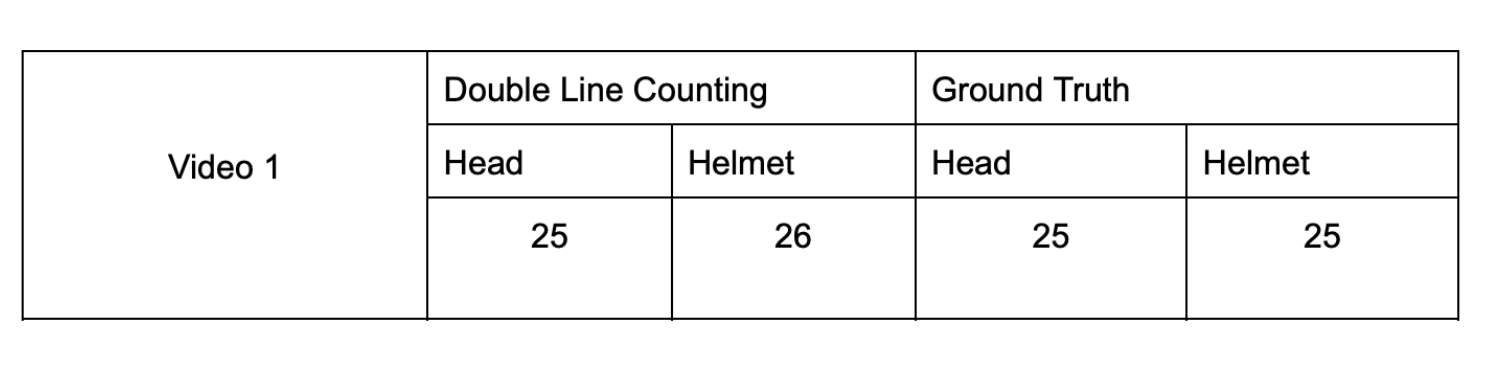
\includegraphics[width=1\textwidth]{test1.png}
\noindent\hspace{2.5em}Table 4.2 shows the counting results for Video 1 using the double-line method compared to the ground truth. The system accurately counted heads (25 vs. 25) but slightly overcounted helmets (26 vs. 25), likely due to duplicate detections or crossing artifacts.


\vspace{0.5em}
\noindent\textbf{Table 4.3} \\
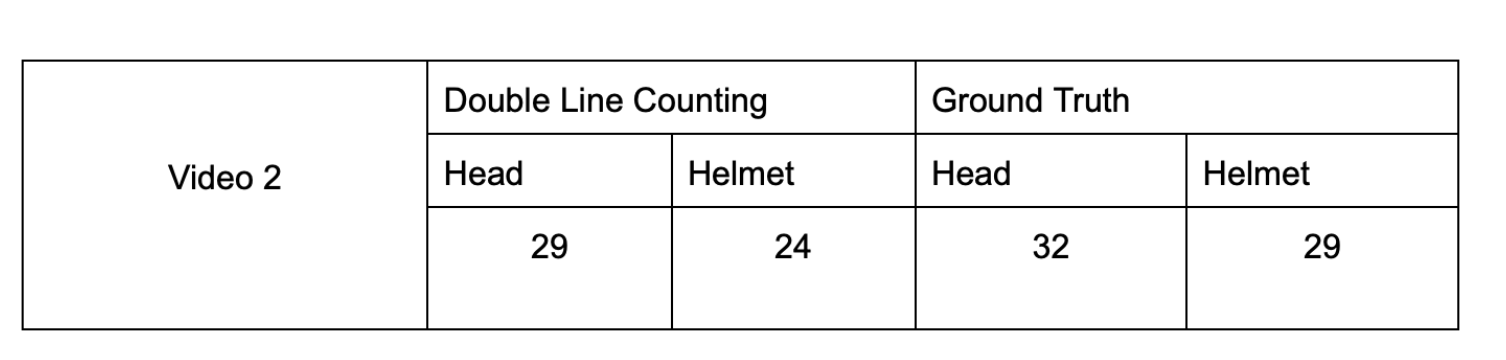
\includegraphics[width=1\textwidth]{test2.png}
\noindent\hspace{2.5em}Table 4.3 shows the double-line counting results for Video 2. The system counted 29 heads and 24 helmets, while the ground truth recorded 32 heads and 29 helmets. This indicates undercounting in both categories, which could be due to missed detections or rapid movements causing objects to skip the counting lines.

\vspace{1em}
For the helmet and head detection specifically, we experimented with adjusting the length of the double-counting lines to evaluate their impact on counting accuracy. For instance, we tested line lengths such as 300 pixels for Line X and 450 pixels for Line Y, along with several other variations. The results indicated that optimal performance occurs when the length of the double lines is kept within approximately 150 pixels. Longer lines tended to increase the likelihood of multiple or false counts due to prolonged object overlap with the counting zone.


\vspace{0.5em}
\noindent\textbf{Table 4.4} \\
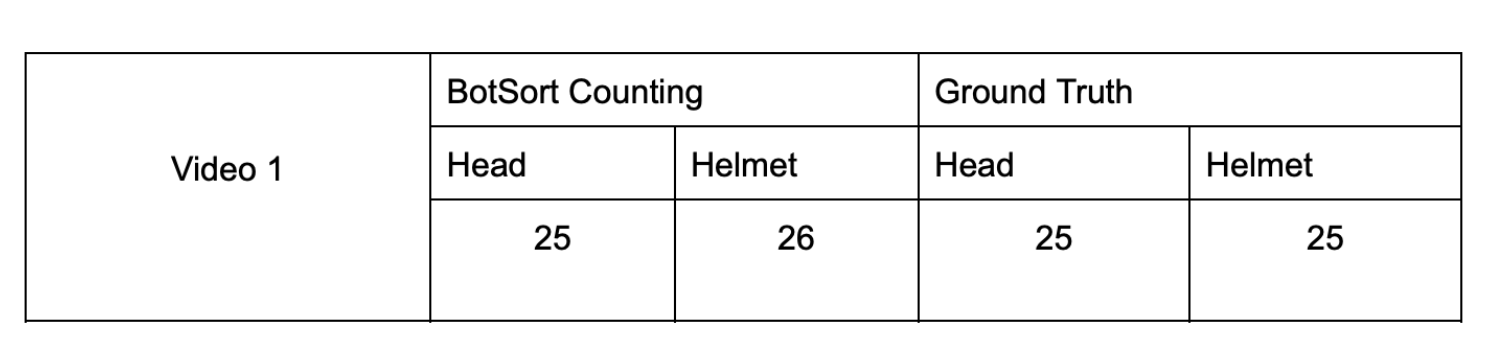
\includegraphics[width=1\textwidth]{test3.png}
\noindent\hspace{2.5em}Table 4.4 presents BotSort counting results for Video 1. The system detected 52 persons and 32 motorbikes, compared to the ground truth values of 51 persons and 30 motorbikes. This reflects a small overcount in both categories, likely due to brief tracking ID switches or overlapping detections in crowded scenes.

\newpage
\vspace{0.5em}
\noindent\textbf{Table 4.5} \\
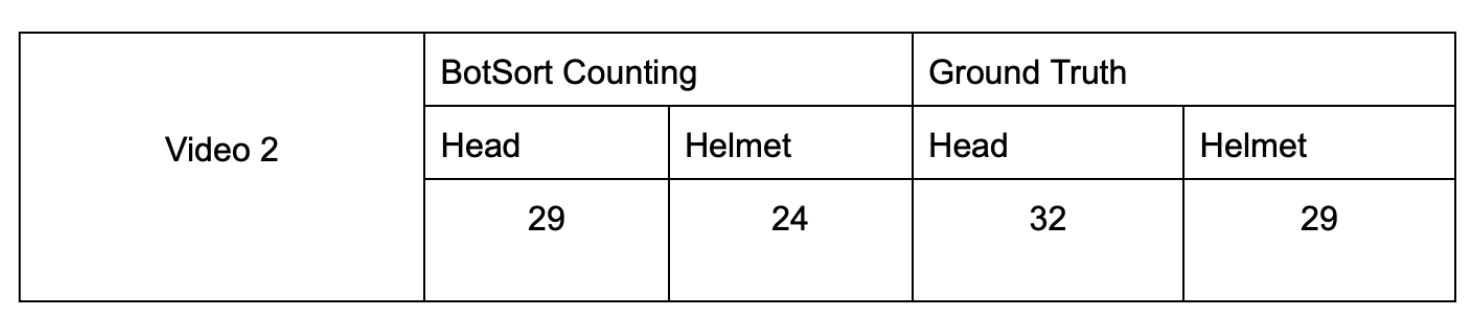
\includegraphics[width=1\textwidth]{test4.png}
\noindent\hspace{2.5em}Table 4.5 summarizes the BotSort results for Video 2. The model counted 56 persons and 44 motorbikes, while the ground truth showed 60 persons and 34 motorbikes. This indicates slight undercounting of persons and significant overcounting of motorbikes, which may result from false positives or tracking drift over longer video durations.


\vspace{1em}
\noindent\hspace{2.5em}In contrast, Tables 4.4 and 4.5 focus on motorbike and person counting accuracy, also based on video 1 and video 2. However, these use the BotSort tracking and counting method instead of the double-line approach. This separation allows us to compare the performance of different counting techniques across differents object categories and scenarios.

\vspace{1em}
\noindent\hspace{2.5em}To evaluate counting accuracy, we use a relative error formula to calculate the percentage difference between the counted value and the ground truth. This approach provides a clear measure of overcounting or undercounting, allowing us to identify and analyze overflow or missed counts in the system.


\vspace{0.5em}
\noindent\textbf{Table 4.6} \\
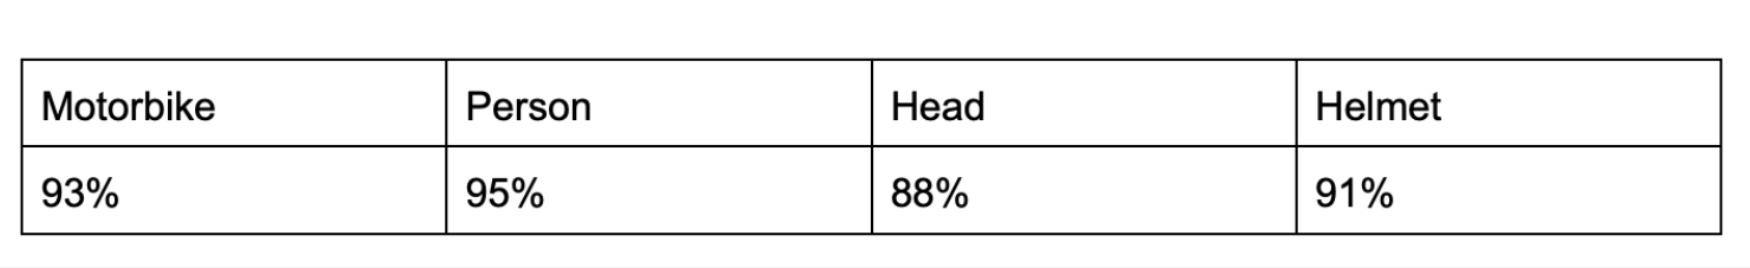
\includegraphics[width=1\textwidth]{conclude_percent.png}

\noindent\hspace{2.5em}Table 4.6 presents the overall performance accuracy of the detection and counting system across four object categories: motorbike, person, head (non-helmeted), and helmet. The results reflect the combined effectiveness of both the object detection model and the counting mechanism (BoT-SORT for motorbike and person, and double-line counting for head and helmet).

The system achieved the highest accuracy in detecting and counting persons (95\%), followed by motorbikes (93\%). These results align with the use of pretrained YOLO models, which provided stable and reliable detection performance. Helmet detection yielded an accuracy of 91\%, demonstrating strong performance from the custom-trained model, especially after multiple iterations and confidence threshold optimization. Head detection (88\%) exhibited slightly lower accuracy, likely due to the challenge of distinguishing non-helmeted heads in varying lighting and occlusion conditions.

Overall, the results confirm that the system performs with high accuracy across all critical object categories, validating its applicability for real-world motorcycle safety monitoring tasks.




